\documentclass[11pt]{article}

% ARR / ACL review mode.  Keep the official template unchanged.
\usepackage[review]{acl}

\usepackage{times}
\usepackage{latexsym}
\usepackage[T1]{fontenc}
\usepackage[utf8]{inputenc}
\usepackage{microtype}
\usepackage{inconsolata}
\usepackage{graphicx}
\usepackage{amsmath}
\usepackage{amssymb}
\usepackage{booktabs}
\usepackage{multirow}
\usepackage{xcolor}
\usepackage{algorithm}
\usepackage{algorithmic}
\usepackage{subcaption}
\usepackage{enumitem}
\usepackage{array}
\usepackage{makecell}
\usepackage{xurl}

\graphicspath{{../../experiments/main_experiment/paper_assets/figures/}}

\newcommand{\samcgs}{SA-MCGS}
\newcommand{\naive}{Naive}
\newcommand{\riskany}{Risk-any}
\newcommand{\riskall}{Risk-all}
\newcommand{\rootthree}{Root@3}
\newcommand{\scc}{SCC}
\newcommand{\oc}{OC}

\title{Collapsing Cyclic Document Graphs into Risk Subgraphs\\
with Structure-Aware Monte Carlo Graph Search}

\author{Anonymous ARR Submission}

\begin{document}
\maketitle

\begin{abstract}
Long documents such as contracts, statutes, software package metadata, and corporate filings often contain risks that are not visible in any single record.  The risk emerges only when mutually dependent records form a cycle: one clause, statute, package, or entity record constrains another, which eventually constrains the first.  Full-context prompting asks an LLM to inspect the entire cycle at once, while standard Monte Carlo tree search is itself unstable on cycles because rollout paths can revisit the same logical state indefinitely.  We propose \samcgs{}, a structure-aware Monte Carlo graph search method that first localizes strongly connected components, then performs local LLM rollouts with relation-first evidence memory, online conformal-style evidence signals, pluggable domain adapters, and a dynamic core that collapses a cyclic region into an inspectable risk subgraph.  We evaluate on a locked critical-stress benchmark covering four authority-backed domains: Debian dependencies, SEC EX-21 subsidiary disclosures, German Civil Code cross-references, and CUAD contracts.  Across 320 model-case pairs and four LLMs, \samcgs{} improves strict \rootthree{} from 48\% to 81\%, \riskany{} from 72\% to 98\%, and \riskall{} from 47\% to 78\%, with zero parse/API failures.  The cost is a lower compression ratio, 53\% versus 67\%, which we show is an expected trade-off for retaining complete critical evidence.
\end{abstract}

\section{Introduction}
\label{sec:intro}

Many high-stakes document analysis tasks are graph problems hidden inside text.  A contract clause may define a deadline, another clause may suspend it, and a later amendment may restore only part of the obligation.  A statute may create an exception whose scope is limited by a distant cross-reference.  A software package may preserve an old interface while a dependent package requires the new one to be present first.  Each record can look plausible in isolation; the risk appears only when the directed dependencies among records are followed.

Large language models (LLMs) can read long contexts, but this does not make them reliable graph reasoners.  Prior work shows that information can be lost in long contexts \citep{liu2024lost}, and legal NLP benchmarks such as CUAD and ContractNLI expose persistent difficulty with evidence that is distributed across non-contiguous clauses \citep{hendrycks2021cuad,koreeda2021contractnli}.  The failure mode we study is sharper: \emph{cyclic} document regions, where evidence is revisitable and diffuse.  A full-\scc{} one-shot prompt may find a suspicious node, but it must simultaneously rank all records, produce a subgraph, and preserve multiple evidence endpoints in one generation.

One might try to escape one-shot prompting by using AlphaGo-style search \citep{silver2016mastering}.  However, standard Monte Carlo tree search assumes that rollouts eventually move forward in a finite tree \citep{kocsis2006bandit}.  In a strongly connected component (\scc{}), paths can revisit the same physical record through many path copies, consuming budget before value estimates stabilize.  Monte Carlo graph search mitigates transpositions in acyclic settings \citep{czech2021monte}, but document cycles require a different unit of reasoning: the cyclic region itself must be localized and collapsed.

We propose \textbf{\samcgs{}}, a structure-aware Monte Carlo graph search method for extracting risk subgraphs from cyclic document regions.  \samcgs{} first finds \scc{} bottlenecks, then performs local window rollouts inside each \scc{}.  Instead of treating risk as an intrinsic property of a single node, it stores relation-first evidence: a node becomes risky when earlier evidence makes its constraint, exception, or handoff incompatible with the graph context.  The final output is a dynamic core risk subgraph that can be inspected or passed upward as a collapsed evaluation point.

Our contributions are:
\begin{itemize}[leftmargin=*,itemsep=2pt]
    \item We formulate \emph{structural risk subgraph extraction}: given a cyclic document subgraph, output a compact subgraph that retains the repair-relevant evidence endpoints, rather than only a single anomalous node.
    \item We introduce \samcgs{}, combining \scc{} localization, local Monte Carlo graph rollouts, relation-first evidence memory, online conformal-style evidence signals, dynamic core compression, and pluggable domain adapters.
    \item We build a locked critical-stress benchmark over four authority-backed domains---Debian, SEC EX-21, BGB, and CUAD---with 320 model-case pairs across GPT-4o, DeepSeek-V3, Qwen2.5-72B, and Gemini 2.5 Pro.
    \item We show that \samcgs{} substantially improves strict \rootthree{}, \riskany{}, and \riskall{} over a full-\scc{} direct-subgraph baseline, while making the compression--retention trade-off explicit.
\end{itemize}

\section{Task Formulation}
\label{sec:formulation}

\paragraph{Record graph.}
Let $G=(V,E)$ be a directed graph whose nodes are document records and whose edges denote typed dependencies such as reference, constraint, modification, trigger, or control.  A record may be a clause, statute section, package metadata entry, subsidiary disclosure, or other domain unit.  We use Tarjan's algorithm \citep{tarjan1972depth} to decompose $G$ into strongly connected components.  A component $S\subseteq V$ is a reasoning bottleneck when every node in $S$ can reach every other node through directed dependencies.

\paragraph{Structural risk.}
We study risks that arise from relations, not merely from suspicious wording.  In the benchmark, an injected critical case modifies existing records only; no new nodes are added.  The core evidence contains a root record, a witness record, and sometimes affected records.  The root and witness can each be locally plausible, but jointly create an incompatible obligation, temporal condition, ownership statement, or dependency handoff.

\paragraph{Output.}
Given a cyclic component $S$, the system returns a risk subgraph $H\subseteq S$ and, when applicable, a ranking over risky records.  We evaluate:
\begin{itemize}[leftmargin=*,itemsep=2pt]
    \item \textbf{\rootthree{}}: whether the injected root appears in the top three ranked records.
    \item \textbf{\riskany{}}: whether $H$ contains at least one repair-relevant risk endpoint.
    \item \textbf{\riskall{}}: whether $H$ retains all core risk endpoints.  This is strict but important for critical risks because remediation often requires seeing both sides of the contradiction.
    \item \textbf{Compression}: $1-|H|/|S|$, reported higher-is-smaller.  Compression is not optimized alone; a tiny subgraph that drops the evidence endpoints is not useful.
\end{itemize}
We also track effective \oc{} discovery as a convergence diagnostic, but do not use it as a main metric because it is cumulative by construction.

\section{Method}
\label{sec:method}

\begin{figure*}[t]
    \centering
    
\includegraphics[width=\textwidth]{fig01_sa_mcgs_framework_architecture.png}
    \caption{\samcgs{} pipeline.  The system builds a directed record graph, localizes cyclic bottlenecks with \scc{} detection, runs local structure-aware rollouts inside each \scc{}, accumulates relation-first evidence, and collapses the component into a dynamic risk core.}
    \label{fig:pipeline}
\end{figure*}

\subsection{Why ordinary MCTS is not enough}
\label{sec:mcts_motivation}

Standard tree search treats a trajectory as a growing path.  In a directed acyclic graph this is acceptable: rollouts eventually terminate and backpropagation updates a finite set of states.  In an \scc{}, the same physical record can be revisited through many path copies, causing three problems: search-tree expansion, rollout truncation, and value dilution.  Table~\ref{tab:mcts_scc} summarizes the motivation study used to design \samcgs{}.

\begin{table}[t]
\centering
\scriptsize
\resizebox{\columnwidth}{!}{%
\begin{tabular}{llrrrr}
\toprule
Method & Topology & Expansion & Trunc. & Q-spread & Hit@3 \\
\midrule
TreeMCTS & DAG & 2.3$\times$ & 0\% & 0.077 & 7\% \\
TreeMCTS & Cycle & 6.4$\times$ & 100\% & 0.044 & 30\% \\
\samcgs{} & Cycle & 1.0$\times$ & -- & 0.371 & 90\% \\
\bottomrule
\end{tabular}
}
\caption{Motivating ablation: ordinary TreeMCTS expands path copies and dilutes value estimates on cyclic dependencies, whereas \samcgs{} treats the \scc{} as a localized reasoning unit.}
\label{tab:mcts_scc}
\end{table}

\subsection{SCC-aware local rollouts}

For each \scc{} $S$, \samcgs{} samples local windows instead of prompting over the entire component in every step.  A window contains visible node text and visible directed edges, and the LLM applies a domain-agnostic risk rubric to produce local risk scores and evidence.  Selection is biased toward records and relations that have accumulated evidence, but the algorithm preserves exploration so that a single early hallucination does not dominate the final core.

\subsection{Relation-first evidence memory}

Early versions of our experiments exposed a weakness in pure node-frequency retention: a node could look harmless until enough prior evidence made it risky.  The final method therefore stores relation-first evidence.  It records not only that node $v$ received a risk score, but also which prior node, edge type, witness, or affected record made $v$ consequential.  Later rollouts can revisit that relation, increase confidence, or evict it if the signal does not persist.

\subsection{Online conformal-style evidence signal}

\samcgs{} uses an online conformal-style signal as a discovery mechanism for ordered-cycle evidence.  The signal is intentionally not a final correctness metric.  Instead, it marks rollouts where local evidence is unusually incompatible with the accumulated history.  This helps route later rollouts toward promising relations and supports convergence analysis.  The final decision is still the retained risk core $H$, evaluated by \riskany{}, \riskall{}, and compression.  Our use follows the broader motivation of conformal calibration under distribution shift \citep{vovk2005algorithmic,gibbs2021adaptive}, but we report empirical retention rather than formal coverage guarantees.

\subsection{Dynamic core compression}

The final risk subgraph is maintained as a dynamic core, not as a monotonically growing set.  New high-confidence evidence can replace weaker evidence; repeated support stabilizes a relation; and the core is constrained by a compression profile.  This design is crucial for critical cases: if a rollout sees both endpoints of a severe contradiction, the core should preserve them even if doing so sacrifices some compression.

\subsection{Pluggable domain adapters}

The search algorithm is domain-general, but record formatting and edge semantics differ across domains.  We therefore expose adapters that provide record serialization, edge saliency hints, and domain-neutral risk wording.  The adapters do not hard-code target error types.  Both \naive{} and \samcgs{} use the same risk semantics: identify structural inconsistency, mutual incompatibility, underspecification, or high-impact risk from visible node text and visible directed edges.

\section{Experimental Setup}
\label{sec:setup}

\subsection{Domains}

We evaluate on four domains chosen for structural diversity and source authority, not for result cherry-picking.  Table~\ref{tab:domains} summarizes their roles.

\begin{table*}[t]
\centering
\small
\begin{tabular}{p{0.13\textwidth}p{0.24\textwidth}p{0.27\textwidth}p{0.25\textwidth}}
\toprule
Domain & Source authority & Graph role & Paper role \\
\midrule
Debian & Package dependency metadata & Software migration / dependency constraints & Non-legal technical generalization \\
SEC EX-21 & Public subsidiary exhibit structure & Entity-control and consolidation paths & Financial/legal entity generalization \\
BGB & German Civil Code references & Statutory cross-reference cycles & Clean legal-rule stress test \\
CUAD & Expert contract review dataset & Long contract clause graph with ambiguity & Noisy contract-domain stress test \\
\bottomrule
\end{tabular}
\caption{Domain coverage.  The benchmark spans technical dependencies, public regulatory disclosures, official statutory references, and expert-labeled commercial contracts.}
\label{tab:domains}
\end{table*}

\subsection{Critical structural injection}

The main experiment uses the locked profile:
\begin{quote}
\small
\texttt{current/default + memory\_stress(structural\_simple\_v2) + critical + 80 SCC blocks/model + 4 models}.
\end{quote}
The injection modifies only existing nodes in a real \scc{}.  Templates include direct mutual exclusion, handoff invariants, temporal gates, and condition triggers.  For example, in BGB a root section can impose a deadline obligation while a distant witness section changes the triggering condition; in CUAD a clause can preserve an operational right while a later clause makes the required condition impossible.  The injected text avoids explicit defect labels.

\subsection{Baselines and models}

The baseline is deliberately strong: \naive{} sees the full \scc{} in one prompt and directly outputs both a whole-\scc{} risk ranking and a risk subgraph.  \samcgs{} sees smaller local windows over 60 rollouts and aggregates evidence into a dynamic core.  Thus \naive{} has more context per call, while \samcgs{} has iterative search and evidence retention.

We evaluate four models: GPT-4o, DeepSeek-V3, Qwen2.5-72B-Instruct, and Gemini 2.5 Pro.  The main data contain 320 model-case pairs and 640 method-level records.  All parse/API failures count as failures in strict metrics.

\section{Main Results}
\label{sec:results}

\begin{table}[t]
\centering
\small
\begin{tabular}{lrr}
\toprule
Metric & \naive{} & \samcgs{} \\
\midrule
\rootthree{} & 48\% & \textbf{81\%} \\
\riskany{} & 72\% & \textbf{98\%} \\
\riskall{} & 47\% & \textbf{78\%} \\
Compression & \textbf{67\%} & 53\% \\
Errors & 59/320 & \textbf{0/320} \\
\bottomrule
\end{tabular}
\caption{Main strict results on 320 model-case pairs.  Parse/API failures are counted in the denominator.}
\label{tab:main}
\end{table}

Table~\ref{tab:main} shows the core result.  \samcgs{} improves \rootthree{} by 33 points, \riskany{} by 26 points, and \riskall{} by 31 points.  The strongest claim is not that one-shot LLMs never find risk; the \naive{} baseline often finds at least one suspicious record.  The difference is that \samcgs{} more reliably preserves the repair-relevant evidence endpoints in the final subgraph.

\begin{figure*}[t]
    \centering
    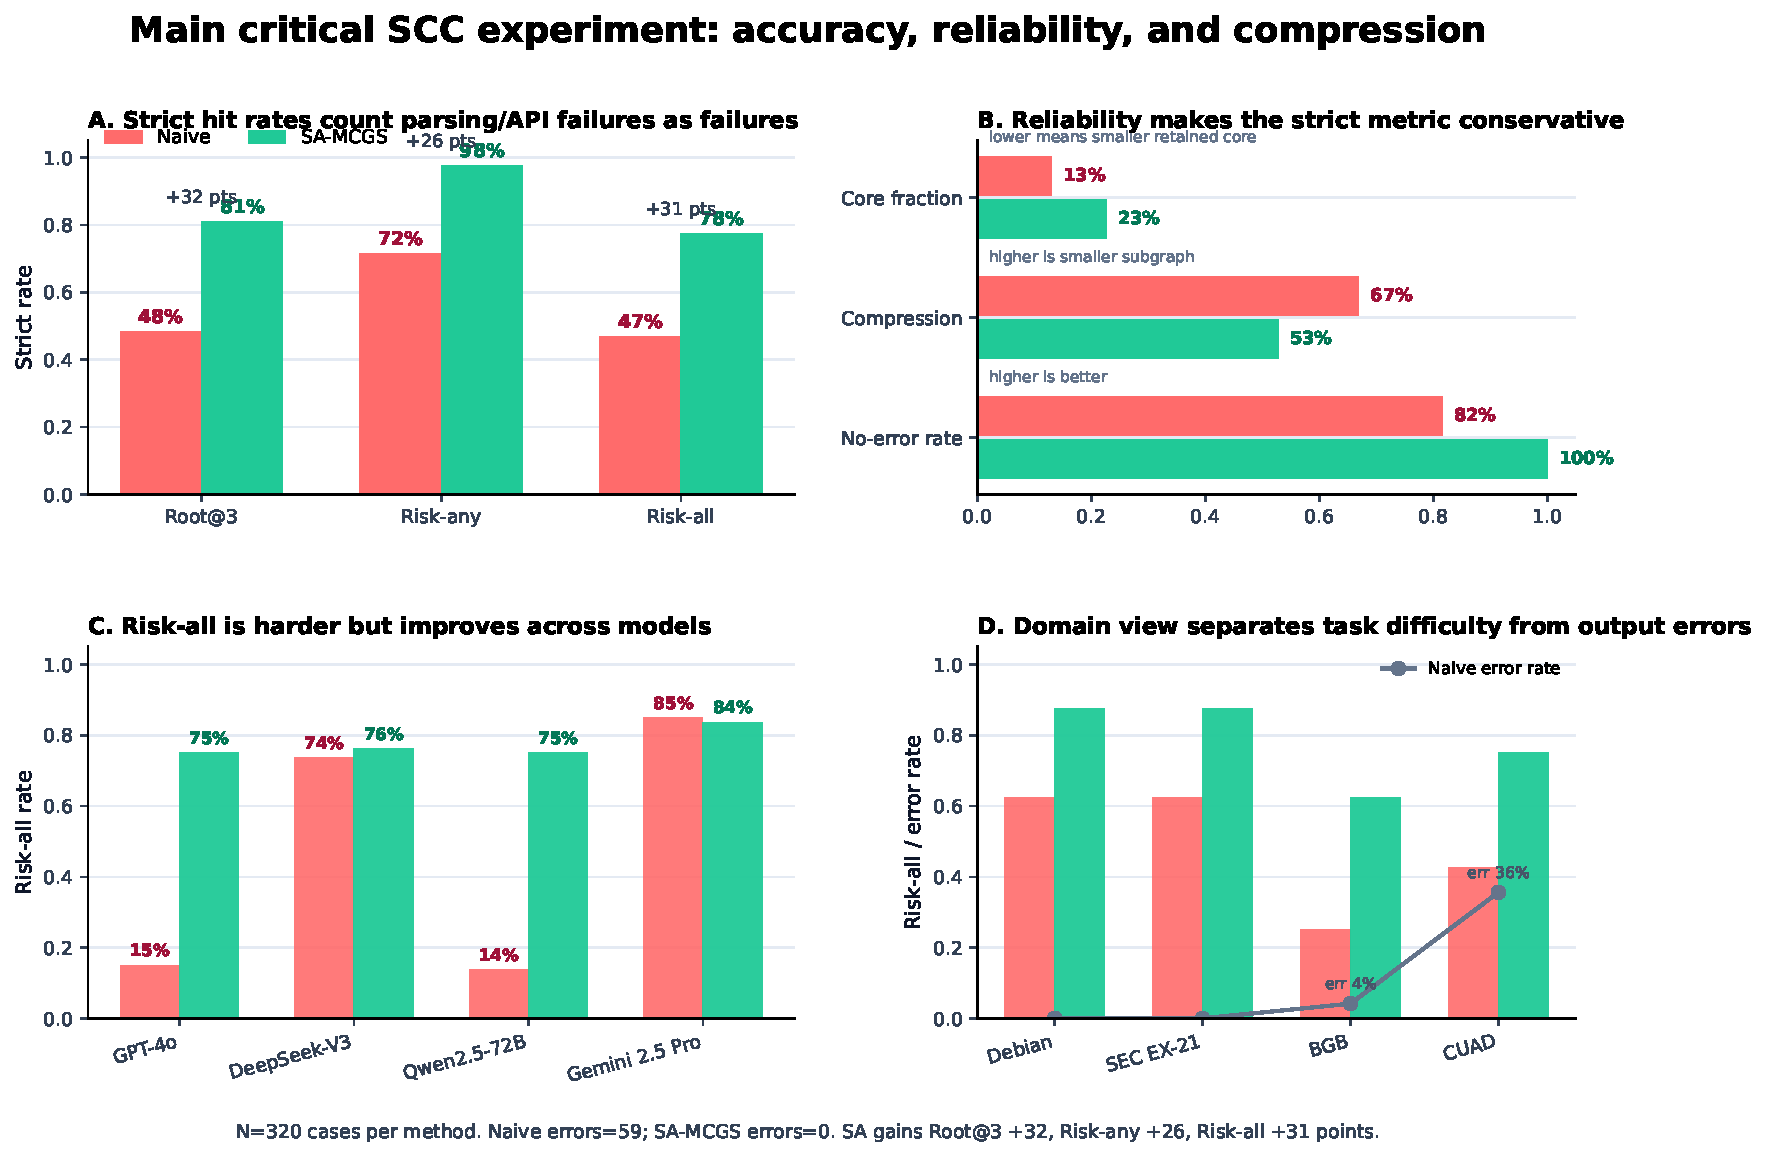
\includegraphics[width=\textwidth]{fig02_main_metrics_strict.pdf}
    \caption{Main critical-\scc{} results.  \samcgs{} improves strict risk localization and endpoint retention, has no parse/API failures, and pays for stronger retention with a larger retained core.}
    \label{fig:main_metrics}
\end{figure*}

The compression row should be read as a trade-off, not a loss.  \naive{} returns smaller subgraphs on average, but it often drops one side of a critical contradiction or fails to return valid structured output.  \samcgs{} deliberately keeps a larger dynamic core when evidence persists across rollouts.

\subsection{Breakdown by model and domain}

The gains are not carried by a single model.  GPT-4o and Qwen2.5-72B show large \riskall{} gains, DeepSeek-V3 is already strong under \naive{} but still improves, and Gemini 2.5 Pro is competitive for both methods.  Domain-wise, CUAD is the hardest setting because long contract text creates high output burden for full-\scc{} prompting; Debian and SEC are cleaner but still show endpoint-retention gains.

\section{Analysis}
\label{sec:analysis}

\subsection{Effect of SCC size}

\begin{figure*}[t]
    \centering
    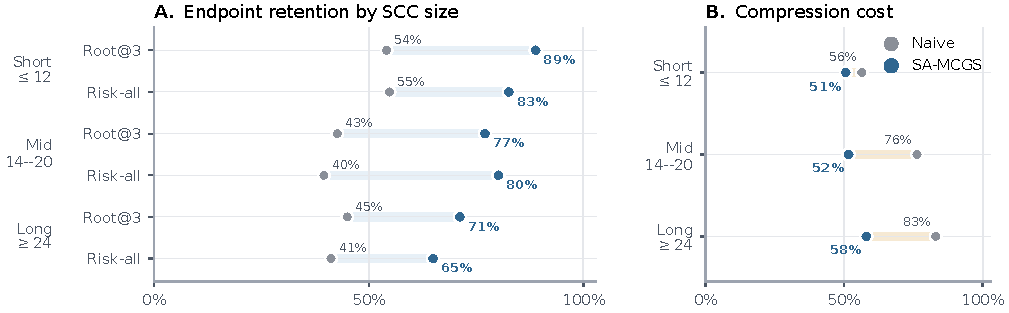
\includegraphics[width=\textwidth]{fig03_main_by_scc_size.pdf}
    \caption{Metrics by \scc{} size.  \samcgs{} remains strongest on endpoint retention across short, mid-sized, and long cyclic components, while very long noisy components make \riskall{} harder for both methods.}
    \label{fig:scc_size}
\end{figure*}

Figure~\ref{fig:scc_size} separates the results by \scc{} size.  In short components ($\leq 12$ nodes), \samcgs{} improves \riskall{} from 55\% to 83\%.  In mid-sized components (14--20 nodes), the improvement is 40\% to 80\%.  In long components ($\geq 24$ nodes), \riskall{} remains difficult, but \samcgs{} still improves 41\% to 65\%.  This is consistent with the task: longer cycles contain more plausible distractors and more native ambiguity, especially in CUAD.

\subsection{Rollout convergence}

\begin{figure*}[t]
    \centering
    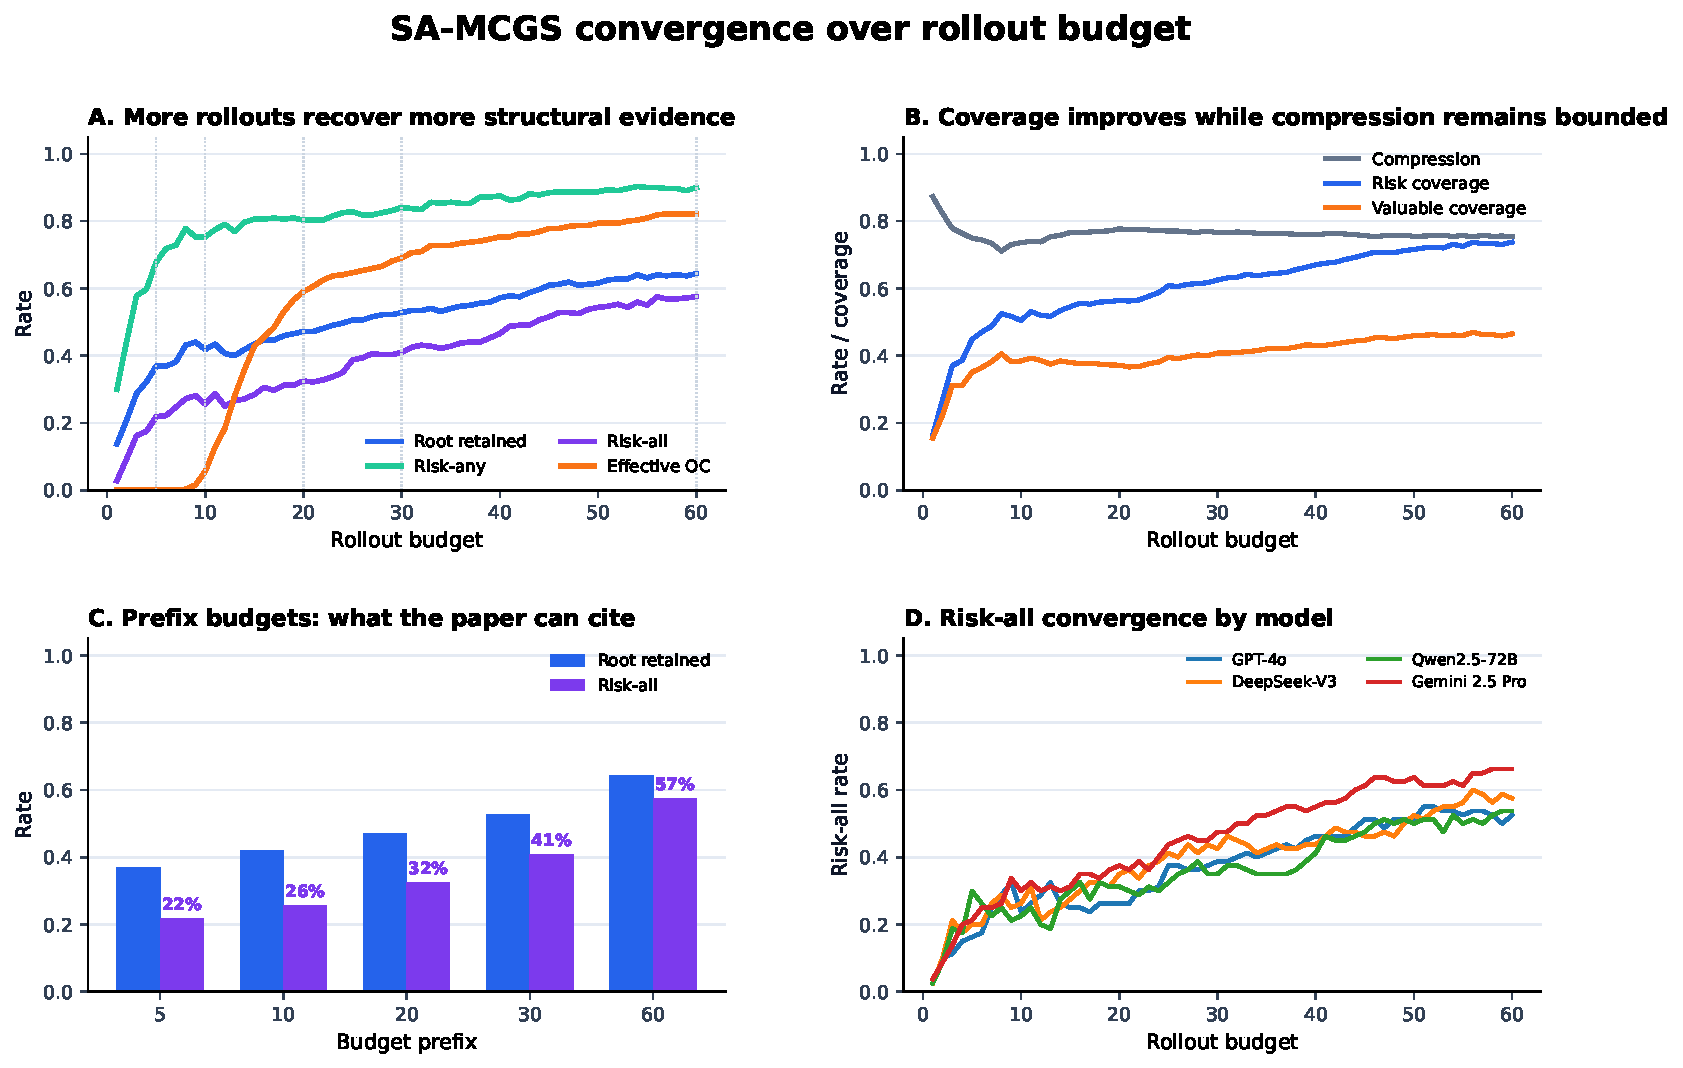
\includegraphics[width=\textwidth]{fig04_budget_prefix_convergence.pdf}
    \caption{Budget-prefix convergence over \samcgs{} rollouts.  \riskany{}, \riskall{}, and risk coverage improve as the rollout budget increases.  Effective \oc{} is cumulative discovery support, not a final metric.}
    \label{fig:convergence}
\end{figure*}

Figure~\ref{fig:convergence} shows that additional rollouts do not merely spend more tokens; they accumulate useful evidence.  At budget 5, \riskall{} is 22\%; at budget 30, it rises to 41\%; at budget 60, it reaches 57\% under prefix reconstruction.  The final run-level \riskall{} in Table~\ref{tab:main} is higher because the dynamic core uses the full retained evidence rather than a simple prefix truncation.  The important trend is that risk coverage and \riskall{} continue to rise well past the first few rollouts, supporting the search interpretation.

\subsection{Compression profile trade-off}

\begin{figure*}[t]
    \centering
    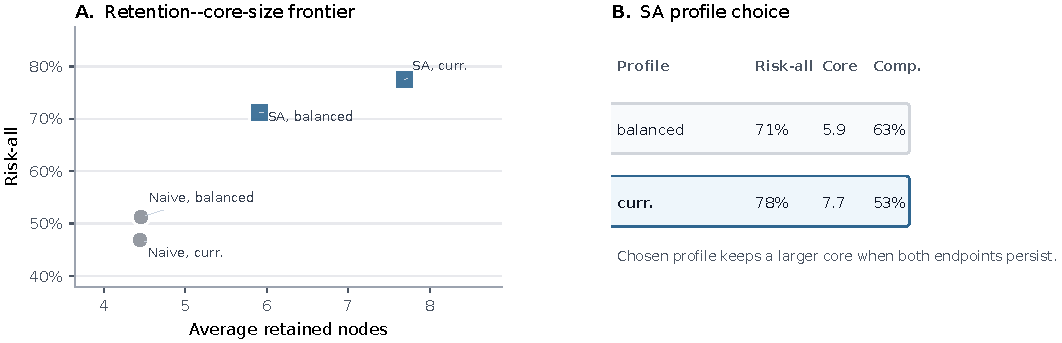
\includegraphics[width=\textwidth]{fig05_compression_profile_tradeoff.pdf}
    \caption{Compression profile ablation.  A more compressed profile yields smaller cores but lowers endpoint retention.  The main paper uses current/default because critical structural risk favors retaining both endpoints over maximizing compression.}
    \label{fig:compression}
\end{figure*}

Figure~\ref{fig:compression} explains why the main experiment uses the current/default compression profile.  A balanced profile increases \samcgs{} compression from 53\% to 63\%, reducing the average retained core from 7.69 to 5.91 nodes.  However, \riskall{} drops from 78\% to 71\%.  For critical risk, we prefer a slightly larger core that preserves both endpoints.

\subsection{Error handling and output burden}

The strict table counts \naive{} failures rather than hiding them.  In the matched no-error subset of 261 comparable pairs, \naive{} improves to 59\% \rootthree{}, 88\% \riskany{}, and 57\% \riskall{}, while \samcgs{} remains higher at 83\%, 98\%, and 77\%.  Therefore the result is not only a JSON stability story.

We also run a CUAD output-burden control in which \naive{} no longer has to produce a full global ranking and per-node evaluations.  This reduces some failures, but long CUAD \scc{}s remain hard: lite \naive{} reaches only 12\% \riskall{} on the controlled long-contract subset.  Full-\scc{} prompting is both a reasoning and an output-structure burden.

\section{Case Study}
\label{sec:case}

\begin{figure*}[t]
    \centering
    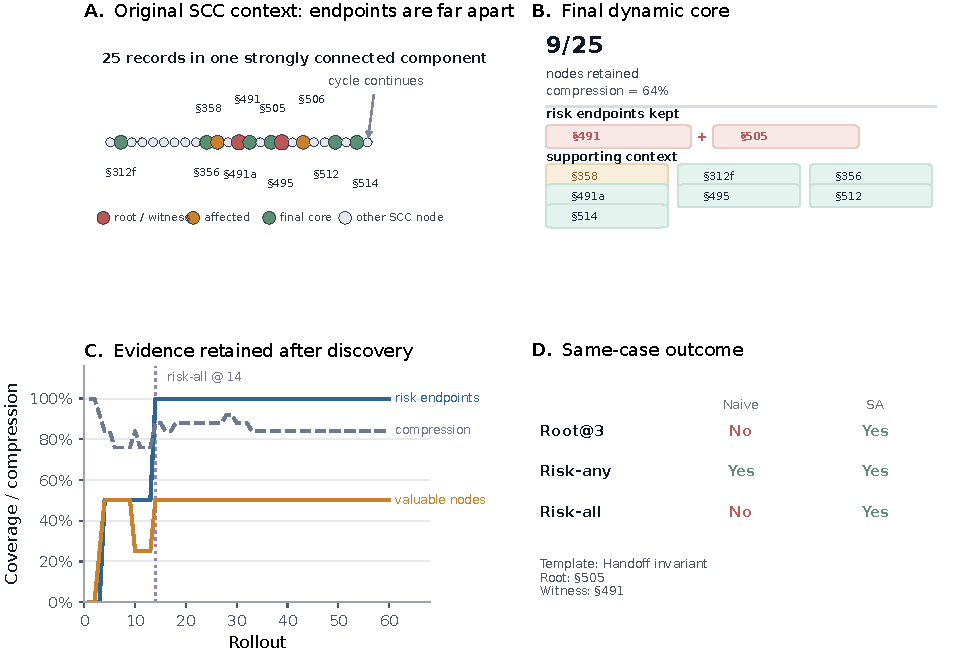
\includegraphics[width=\textwidth]{fig06_representative_scc_collapse.pdf}
    \caption{Representative BGB case.  The root and witness are far apart in a 25-node statutory-reference \scc{}.  \samcgs{} retains both endpoints in a 9-node dynamic core and succeeds where the full-\scc{} \naive{} baseline misses \rootthree{} and \riskall{}.}
    \label{fig:case}
\end{figure*}

Figure~\ref{fig:case} illustrates the intended use of the method.  The original \scc{} is too large to treat as a single atomic finding, yet too cyclic for ordinary path search.  \samcgs{} localizes the evidence through rollouts, then returns a core containing the root, witness, and affected records.  This is more useful for review than a single node label: a human can inspect the retained endpoints and decide how the conflict should be repaired.

\section{Related Work}
\label{sec:related}

\paragraph{LLM reasoning and long context.}
Chain-of-thought prompting improves sequential reasoning \citep{wei2022chain}, but cyclic document risk requires revisiting and reconciling multiple records rather than extending one chain.  Long-context studies show that models can fail to use information reliably throughout a context \citep{liu2024lost}.  Legal NLP datasets such as CUAD and ContractNLI motivate document-level reasoning, but they do not by themselves solve cyclic evidence retention \citep{hendrycks2021cuad,koreeda2021contractnli}.

\paragraph{Search-augmented LLMs.}
Tree of Thoughts \citep{yao2024tree}, Graph of Thoughts \citep{besta2024graph}, and planning-style LLM search \citep{hao2023reasoning} demonstrate that explicit search can improve reasoning.  \samcgs{} differs by operating on externally constructed document graphs and by treating \scc{}s as topological bottlenecks that must be collapsed into risk subgraphs.

\paragraph{Monte Carlo search on graphs.}
MCTS and AlphaGo-style search are powerful when the search space has stable state transitions \citep{silver2016mastering,kocsis2006bandit}.  Monte Carlo graph search reuses transpositions in graph settings \citep{czech2021monte}, while work on uncertainty in MCTS highlights the difficulty of loops \citep{moerland2020mcts}.  Our method is motivated by this gap: cyclic document regions require information-preserving \scc{} handling rather than ordinary tree expansion.

\paragraph{Graph legal analysis and calibration.}
Network analysis has been used to study statutory cross-references \citep{boulet2021measuring}, and contract graph extraction is an active direction \citep{dechtiar2025graphgrpolex}.  \samcgs{} is complementary: it assumes a record graph is available and focuses on risk search inside cyclic components.  We use conformal prediction ideas \citep{vovk2005algorithmic,gibbs2021adaptive} as inspiration for online evidence calibration, while reporting empirical discovery and retention metrics.

\section*{Limitations}
\label{sec:limitations}

\samcgs{} is more expensive than one-shot prompting because it performs many local LLM calls.  The method is intended for high-risk cyclic components, not every record in a document.  Our benchmark uses injected critical risks so that ground truth is controlled; naturally occurring risks may be messier and require human audit.  Graph construction quality also matters: missing or spurious edges can change the \scc{}s that the method receives.  Finally, \riskall{} remains difficult in noisy long-contract settings, which is why we report it explicitly rather than replacing it with the easier \riskany{} metric.

\section*{Ethics Statement}
\label{sec:ethics}

This work targets decision support for expert review, not automated legal, financial, or software-security decisions.  The output is an inspectable risk subgraph rather than an ungrounded verdict, and the intended workflow keeps a human reviewer responsible for final judgment.  The evaluated sources are public or benchmark data.  The main ethical risk is over-reliance: a missed endpoint or a graph-construction error can still matter in high-stakes review.  We therefore report strict failures, compression trade-offs, and planned human-audit materials rather than presenting the system as a replacement for experts.

\section{Conclusion}
\label{sec:conclusion}

We introduced \samcgs{}, a structure-aware Monte Carlo graph search method for cyclic document risk.  The central idea is to stop treating a long \scc{} as either a flat prompt or an ordinary tree-search path.  Instead, \samcgs{} localizes the \scc{}, searches it through local rollouts, stores relation-first evidence, and collapses the component into a dynamic risk core.  Across four domains and four LLMs, this yields substantially stronger root localization and endpoint retention than a full-\scc{} direct-subgraph baseline, while making the cost in compression explicit.

\bibliography{custom}

\appendix

\section{Additional Experimental Details}
\label{sec:appendix_experiments}

\begin{table*}[t]
\centering
\small
\begin{tabular}{llrrrrrr}
\toprule
Model & Method & N & Errors & \rootthree{} & \riskany{} & \riskall{} & Compression \\
\midrule
GPT-4o & \naive{} & 80 & 17 & 26\% & 55\% & 15\% & 68\% \\
GPT-4o & \samcgs{} & 80 & 0 & 86\% & 100\% & 75\% & 51\% \\
DeepSeek-V3 & \naive{} & 80 & 0 & 75\% & 88\% & 74\% & 70\% \\
DeepSeek-V3 & \samcgs{} & 80 & 0 & 80\% & 95\% & 76\% & 51\% \\
Qwen2.5-72B & \naive{} & 80 & 41 & 2\% & 46\% & 14\% & 43\% \\
Qwen2.5-72B & \samcgs{} & 80 & 0 & 70\% & 98\% & 75\% & 53\% \\
Gemini 2.5 Pro & \naive{} & 80 & 1 & 90\% & 98\% & 85\% & 75\% \\
Gemini 2.5 Pro & \samcgs{} & 80 & 0 & 88\% & 98\% & 84\% & 56\% \\
\bottomrule
\end{tabular}
\caption{Model-level strict breakdown.}
\label{tab:model_breakdown}
\end{table*}

\begin{table*}[t]
\centering
\small
\begin{tabular}{llrrrrrr}
\toprule
Domain & Method & N & Errors & \rootthree{} & \riskany{} & \riskall{} & Compression \\
\midrule
Debian & \naive{} & 32 & 0 & 41\% & 94\% & 62\% & 56\% \\
Debian & \samcgs{} & 32 & 0 & 84\% & 100\% & 88\% & 53\% \\
SEC EX-21 & \naive{} & 80 & 0 & 64\% & 99\% & 62\% & 59\% \\
SEC EX-21 & \samcgs{} & 80 & 0 & 96\% & 100\% & 88\% & 50\% \\
BGB & \naive{} & 48 & 2 & 25\% & 67\% & 25\% & 62\% \\
BGB & \samcgs{} & 48 & 0 & 75\% & 98\% & 62\% & 52\% \\
CUAD & \naive{} & 160 & 57 & 49\% & 55\% & 42\% & 79\% \\
CUAD & \samcgs{} & 160 & 0 & 74\% & 96\% & 75\% & 54\% \\
\bottomrule
\end{tabular}
\caption{Domain-level strict breakdown.  CUAD contributes the largest number of long, noisy contract cases and most \naive{} parse failures.}
\label{tab:domain_breakdown}
\end{table*}

\begin{table}[t]
\centering
\small
\resizebox{\columnwidth}{!}{%
\begin{tabular}{llrrr}
\toprule
Scope & Method & N & \rootthree{} & \riskall{} \\
\midrule
Strict & \naive{} & 320 & 48\% & 47\% \\
Strict & \samcgs{} & 320 & 81\% & 78\% \\
Valid-only & \naive{} & 261 & 59\% & 57\% \\
Matched no-error & \naive{} & 261 & 59\% & 57\% \\
Matched no-error & \samcgs{} & 261 & 83\% & 77\% \\
\bottomrule
\end{tabular}
}
\caption{Error-handling analysis.  The main table uses strict rates; matched no-error rates show that the difference is not only parse stability.}
\label{tab:error_handling}
\end{table}

\begin{figure*}[t]
    \centering
    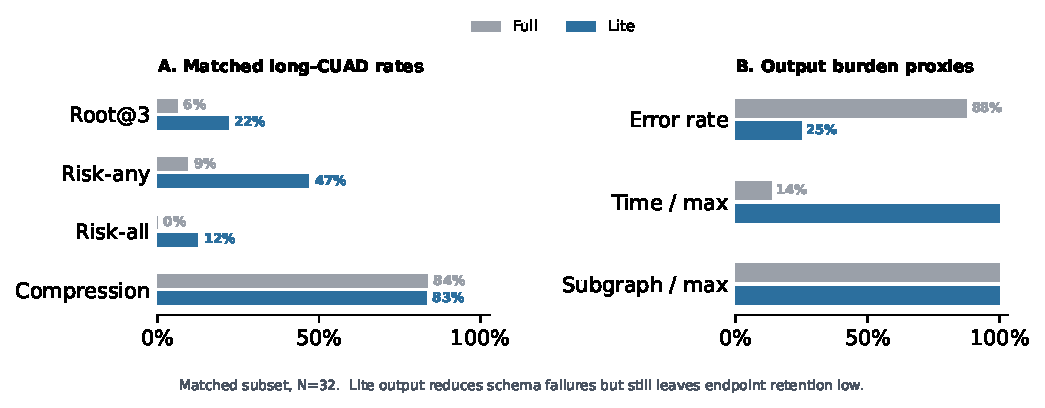
\includegraphics[width=.85\textwidth]{figA2_naive_output_burden.pdf}
    \caption{Naive output-burden control.  Reducing the output schema helps full-\scc{} prompting, but does not close the endpoint-retention gap on long CUAD components.}
    \label{fig:naive_burden}
\end{figure*}

\section{Prompt Parity}
\label{sec:appendix_prompt_parity}

The formal experiments use a shared domain-agnostic risk semantics.  The difference between methods is the inference interface: \naive{} applies the rubric once to the full \scc{}, while \samcgs{} applies it repeatedly to local windows and aggregates evidence.  The shared rubric is:

\begin{quote}
\small
Analyze a directed graph of interdependent records.  Each node contains a record.  Each directed edge indicates that one record depends on, constrains, references, modifies, or otherwise affects another record.  A record or relation is risky if it is structurally inconsistent, mutually incompatible, underspecified, or high-impact under the visible graph context.  Use only visible node text and visible directed edges, and explain concrete conflicts using exact record IDs.
\end{quote}

\section{Human Audit Materials}
\label{sec:appendix_human}

We prepared a human annotation package under \path{experiments/main_experiment/paper_assets/human_annotation_pack/}.  The expert-facing pack contains a curated 12-case sample, per-case materials, and a bilingual HTML interface that supports in-page annotation, node-level evidence popups, and Excel export.  The human audit is intentionally separated from the automatic main table and will be reported as an additional validation layer.

\end{document}
